\section{Results}\label{sec:results}

\subsection{A spatially aware baseline fails in the reference-preserving setting}\label{sec:res_spatial}
Table~\ref{tab:graphst} compares \frost with GraphST on a common subsample of 10{,}000 source and 10{,}000
reference cells per pair. \frost transfers labels more accurately than GraphST (median paired difference $+0.376$,
$n=12$, $p=0.0005$, the smallest value attainable with 12 pairs). Mixing does not differ significantly
($+0.092$, $n=12$, $p=0.064$). GraphST therefore loses label transfer without gaining mixing in exchange.

GraphST is also worse than performing no alignment at all. Its transfer is lower than that of the unaligned
embeddings (mean difference $-0.243$, $n=12$, $p=0.0015$), and its only gain over them is in mixing ($+0.377$,
$n=12$, $p=0.0005$). This is the signature of over-correction: the platforms become harder to tell apart because
cell-type structure has been destroyed. \frost, by contrast, improves on no alignment in both transfer ($p=0.0010$)
and mixing ($p=0.0005$; $n=12$ for both).

The reference itself moves. GraphST re-embeds both sections, and the 15-NN neighbourhoods of reference cells
overlap little with those before integration (drift 0.966--0.989 across pairs, mean 0.979). Any classifier,
annotation or index built on the reference would have to be rebuilt. For \frost and every other reference-preserving
method, drift is exactly zero. This is a property of the architecture, not of tuning.

Scale differs as well. GraphST had to be run on 10{,}000 cells per side because its dense spatial adjacency
exhausted memory at 90{,}000 cells, whereas \frost runs on the full 40{,}000--45{,}000 cells per side.
GraphST was run once, at its published defaults; Section~\ref{sec:limitations} discusses what this comparison does
and does not establish. Wall-clock time for GraphST was not extracted~\todo{GraphST wall-clock from log 42}.

\begin{table}[t]
\centering
\caption{Comparison with a spatially aware baseline on a common subsample (10{,}000 + 10{,}000 cells per pair,
12 pairs, seed 0). Means over pairs. Metrics are defined in Section~\ref{sec:metrics} and are not comparable with
those of Table~\ref{tab:main}. ``Wins'' counts the pairs in which a method has the highest transfer.}
\label{tab:graphst}
\small
\begin{tabular}{@{}lcccc@{}}
\toprule
Method & Transfer $\uparrow$ & Mixing $\uparrow$ & Reference drift $\downarrow$ & Wins (transfer) \\
\midrule
GraphST            & 0.3731 & 0.3982 & 0.979 & 0 \\
No alignment (raw) & 0.6162 & 0.0208 & 0.000 & 1 \\
USHER-ST           & 0.7133 & 0.3206 & 0.000 & 1 \\
\frost w/o CORAL   & 0.7142 & 0.3218 & 0.000 & 2 \\
USHER-CC           & 0.7219 & 0.5117 & 0.000 & 2 \\
\frost             & \textbf{0.7223} & \textbf{0.5158} & 0.000 & \textbf{6} \\
\bottomrule
\end{tabular}
\end{table}

\subsection{Benchmark against reference-preserving and reference-modifying baselines}\label{sec:res_bench}
Figure~\ref{fig:grid} shows all 16 metrics per source technology (per tissue in Supplementary
Figure~\ref{fig:grid_tissue}). Because batch\_v2 and bio\_v2 are means of the metrics beside them, ranking all 16
would count the same information several times. We therefore summarise with a compact set (Table~\ref{tab:main}):
the two group scores, their weighted total, and the four task metrics. On all seven, \frost ranks among the top
three of 11 methods. It is first on xfer\_all; second on batch\_v2, total\_v2, rare\_purity and knn\_xen; third on
bio\_v2 and xfer\_main. Where \frost is not first, the leader is usually one of its own ablations. USHER-CC leads
batch\_v2, total\_v2 and rare\_purity; USHER-ST, which has no CORAL step, leads xfer\_main and knn\_xen. The one
baseline that leads a column is ridge on bio\_v2. Table~\ref{tab:main} also reports gene imputation under the
original protocol, where \frost ranks second. That advantage exists only under a protocol that leaks the predicted
gene; Section~\ref{sec:limitations} explains why it reverses once the leak is removed.

Figure~\ref{fig:gaps} gives the paired tests against every baseline. We call a difference significant at $p<0.05$
(exact Wilcoxon) and otherwise report no significant difference. Ridge is the informative comparison, because it uses
the same auxiliary labels and the same moment matching as \frost and differs mainly in how source cells are paired
with reference cells. \frost exceeds ridge on batch\_v2 ($n=12$, $p=0.0005$), total\_v2 ($n=12$, $p=0.0005$) and
knn\_xen ($n=12$, $p=0.0015$). It does not differ significantly on bio\_v2 (median $-0.006$, $n=12$, $p=0.06$; ridge
slightly higher), xfer\_main ($n=12$, $p=0.29$), xfer\_all ($n=11$, $p=0.64$) or rare\_purity ($n=12$, $p=0.68$).
The total\_v2 result is not independent evidence. batch\_v2 ranges from 0.34 to 0.66 across methods and bio\_v2
only from 0.60 to 0.69, so differences in total\_v2 are driven by mixing. The knn\_xen advantage is specific to
ridge: \frost does not differ significantly from centring ($p=0.79$) or Harmony ($p=0.62$) on that metric. Read as a
Pareto trade-off rather than through a composite score, \frost gains in mixing over ridge with no significant loss
in conservation or transfer.

Against the simpler baselines the picture is consistent. \frost exceeds per-assay centring on batch\_v2, bio\_v2,
total\_v2, xfer\_all and rare\_purity. It does not differ significantly on xfer\_main ($p=0.27$) or knn\_xen
($p=0.79$). It exceeds Harmony on every compact metric except knn\_xen ($p=0.62$). It exceeds Symphony, the published
reference-mapping method, on all seven ($p$ between 0.0005 and 0.034); part of that gap may reflect Symphony's
own count-based representation (Section~\ref{sec:baselines}).

\begin{table}[t]
\centering
\caption{Compact benchmark: means over 12 pairs (three seeds for stochastic methods). Methods marked $^{*}$ modify
the reference embedding. Best per column in bold.
$^{\dagger}$Original imputation protocol, which leaks the predicted gene into the source embedding; under the
leakage-controlled protocol standard baselines exceed every USHER-family variant in 11 of 12 pairs
(Section~\ref{sec:limitations}). Symphony is not scored on imputation.}
\label{tab:main}
\small
\setlength{\tabcolsep}{4pt}
\begin{tabular}{@{}lcccccccc@{}}
\toprule
Method & batch\_v2 & bio\_v2 & total\_v2 & xfer\_main & xfer\_all & rare\_purity & knn\_xen & imput.$^{\dagger}$ \\
\midrule
raw        & 0.3448 & 0.5956 & 0.4953 & 0.5972 & 0.3256 & 0.1547 & 0.3061 & 0.0955 \\
center     & 0.4419 & 0.6240 & 0.5511 & 0.6778 & 0.4066 & 0.2290 & 0.3308 & 0.1073 \\
CORAL      & 0.5939 & 0.6605 & 0.6339 & 0.6397 & 0.4027 & 0.2527 & 0.3088 & 0.0919 \\
MNN-ref    & 0.4258 & 0.6197 & 0.5421 & 0.6383 & 0.3619 & 0.1814 & 0.3182 & 0.1034 \\
ridge      & 0.5447 & \textbf{0.6874} & 0.6303 & 0.6867 & 0.4266 & 0.2623 & 0.3101 & 0.0620 \\
Harmony$^{*}$   & 0.4499 & 0.6204 & 0.5522 & 0.6512 & 0.3716 & 0.2012 & 0.3210 & 0.1068 \\
Scanorama$^{*}$ & 0.3843 & 0.6110 & 0.5203 & 0.6050 & 0.3422 & 0.1702 & 0.3089 & 0.0956 \\
Symphony$^{*}$  & 0.4861 & 0.6099 & 0.5604 & 0.4949 & 0.2990 & 0.1841 & 0.2470 & -- \\
USHER-ST   & 0.5479 & 0.6763 & 0.6249 & \textbf{0.6913} & 0.4074 & 0.2267 & \textbf{0.3372} & \textbf{0.1150} \\
USHER-CC   & \textbf{0.6600} & 0.6813 & \textbf{0.6728} & 0.6896 & 0.4288 & \textbf{0.2652} & 0.3322 & 0.1096 \\
\frost     & 0.6593 & 0.6811 & 0.6724 & 0.6891 & \textbf{0.4291} & 0.2642 & 0.3330 & 0.1145 \\
\bottomrule
\end{tabular}
\end{table}

\begin{figure}[p]
\centering
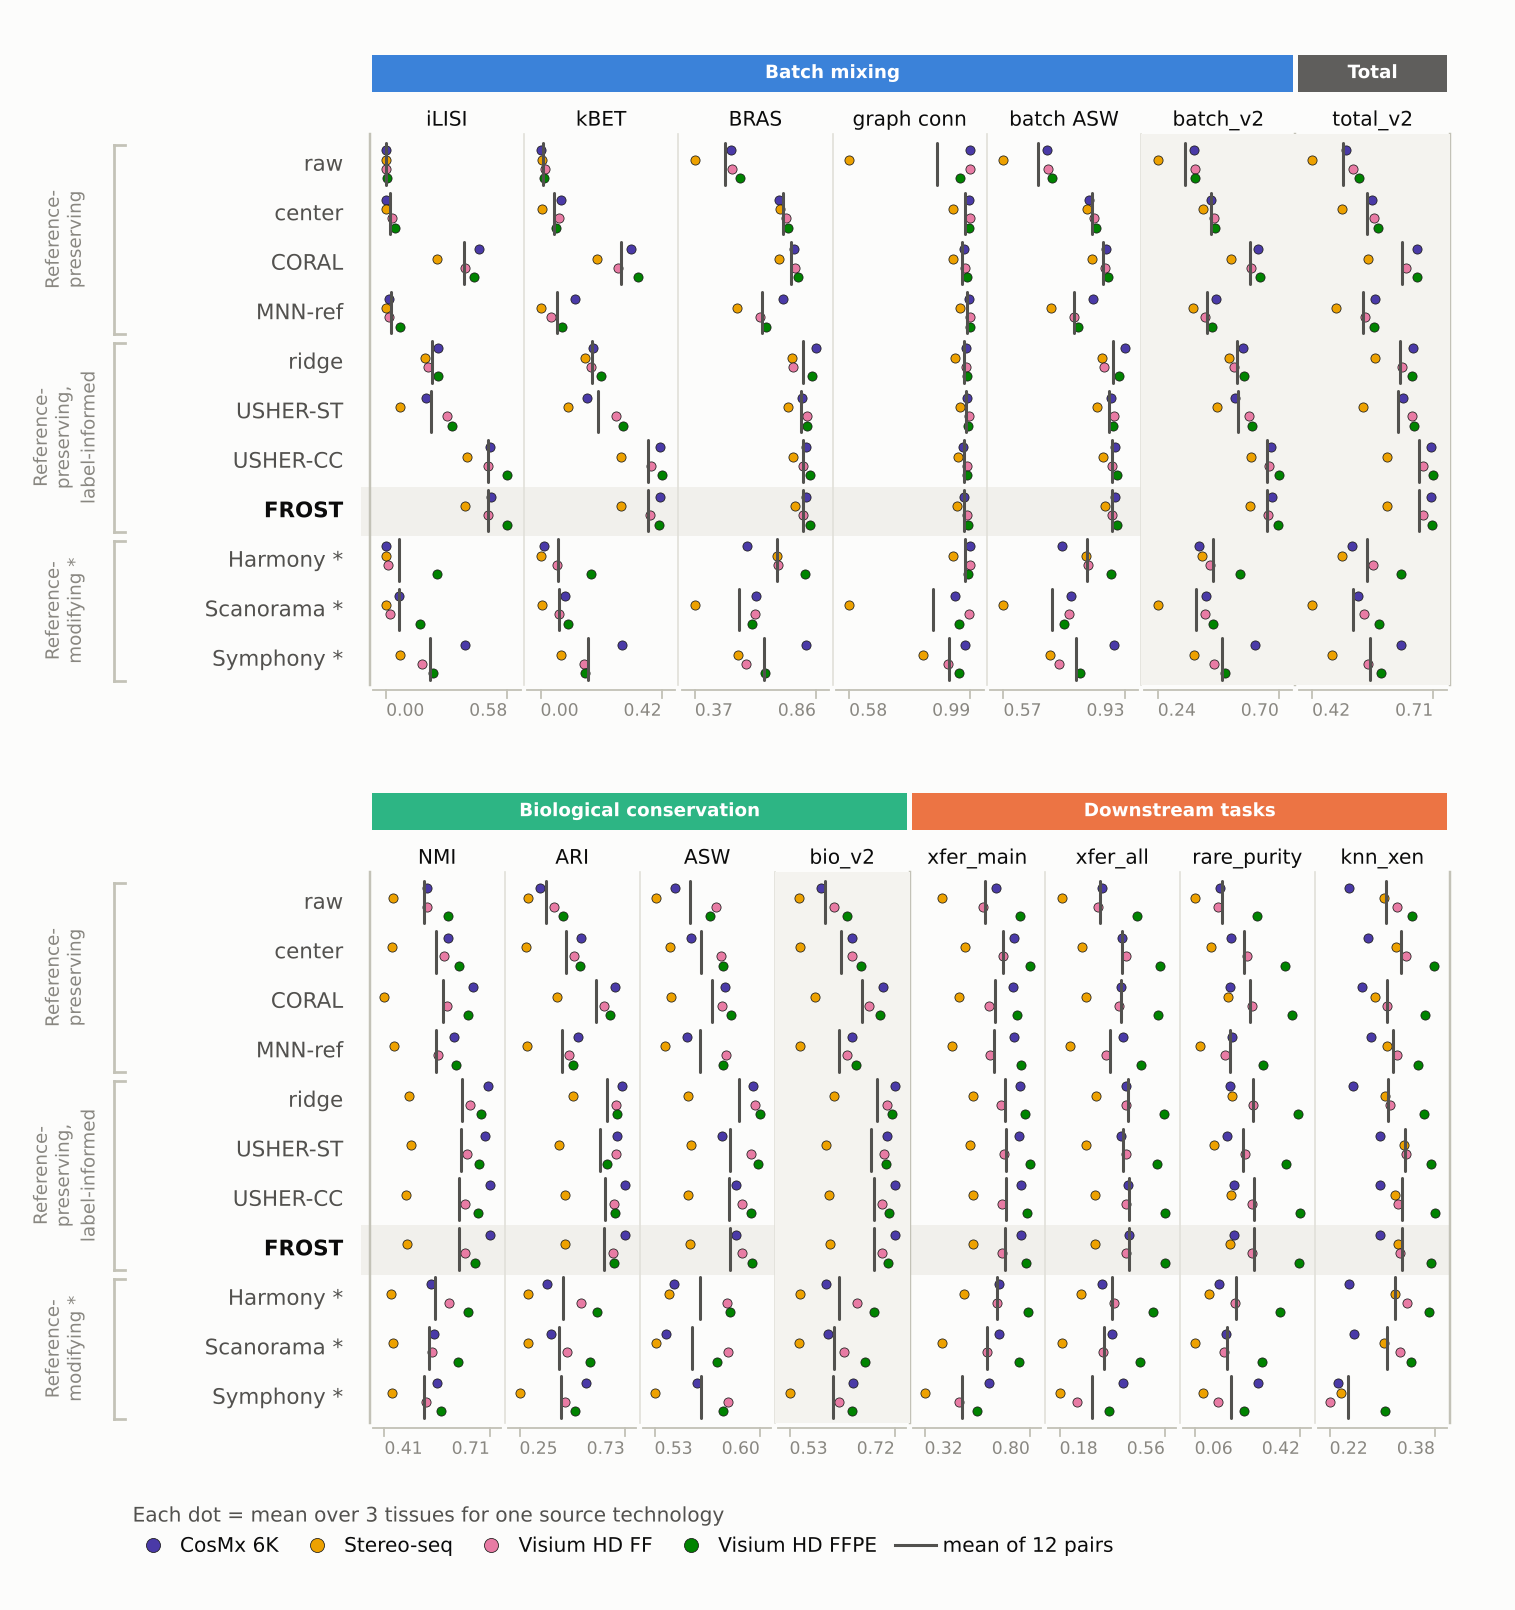
\includegraphics[width=\linewidth]{figs/fig_grid_tech.png}
\caption{All 16 metrics, 11 methods. Each dot is the mean over three tissues for one source technology; the vertical
bar is the mean over 12 pairs. Axes span the observed range of each metric, without min--max scaling across
methods. Shaded columns are group scores of the metrics to their left: batch\_v2 is the mean of iLISI, kBET, BRAS
and graph connectivity; bio\_v2 the mean of NMI, ARI, ASW, cLISI and isolated labels; total\_v2 $=0.4\,$batch\_v2
$+\,0.6\,$bio\_v2. $^{*}$Methods that modify the reference embedding. The four pairs of a tissue share a reference
and a patient, so the 12 pairs are not independent.}
\label{fig:grid}
\end{figure}

\begin{figure}[!t]
\centering
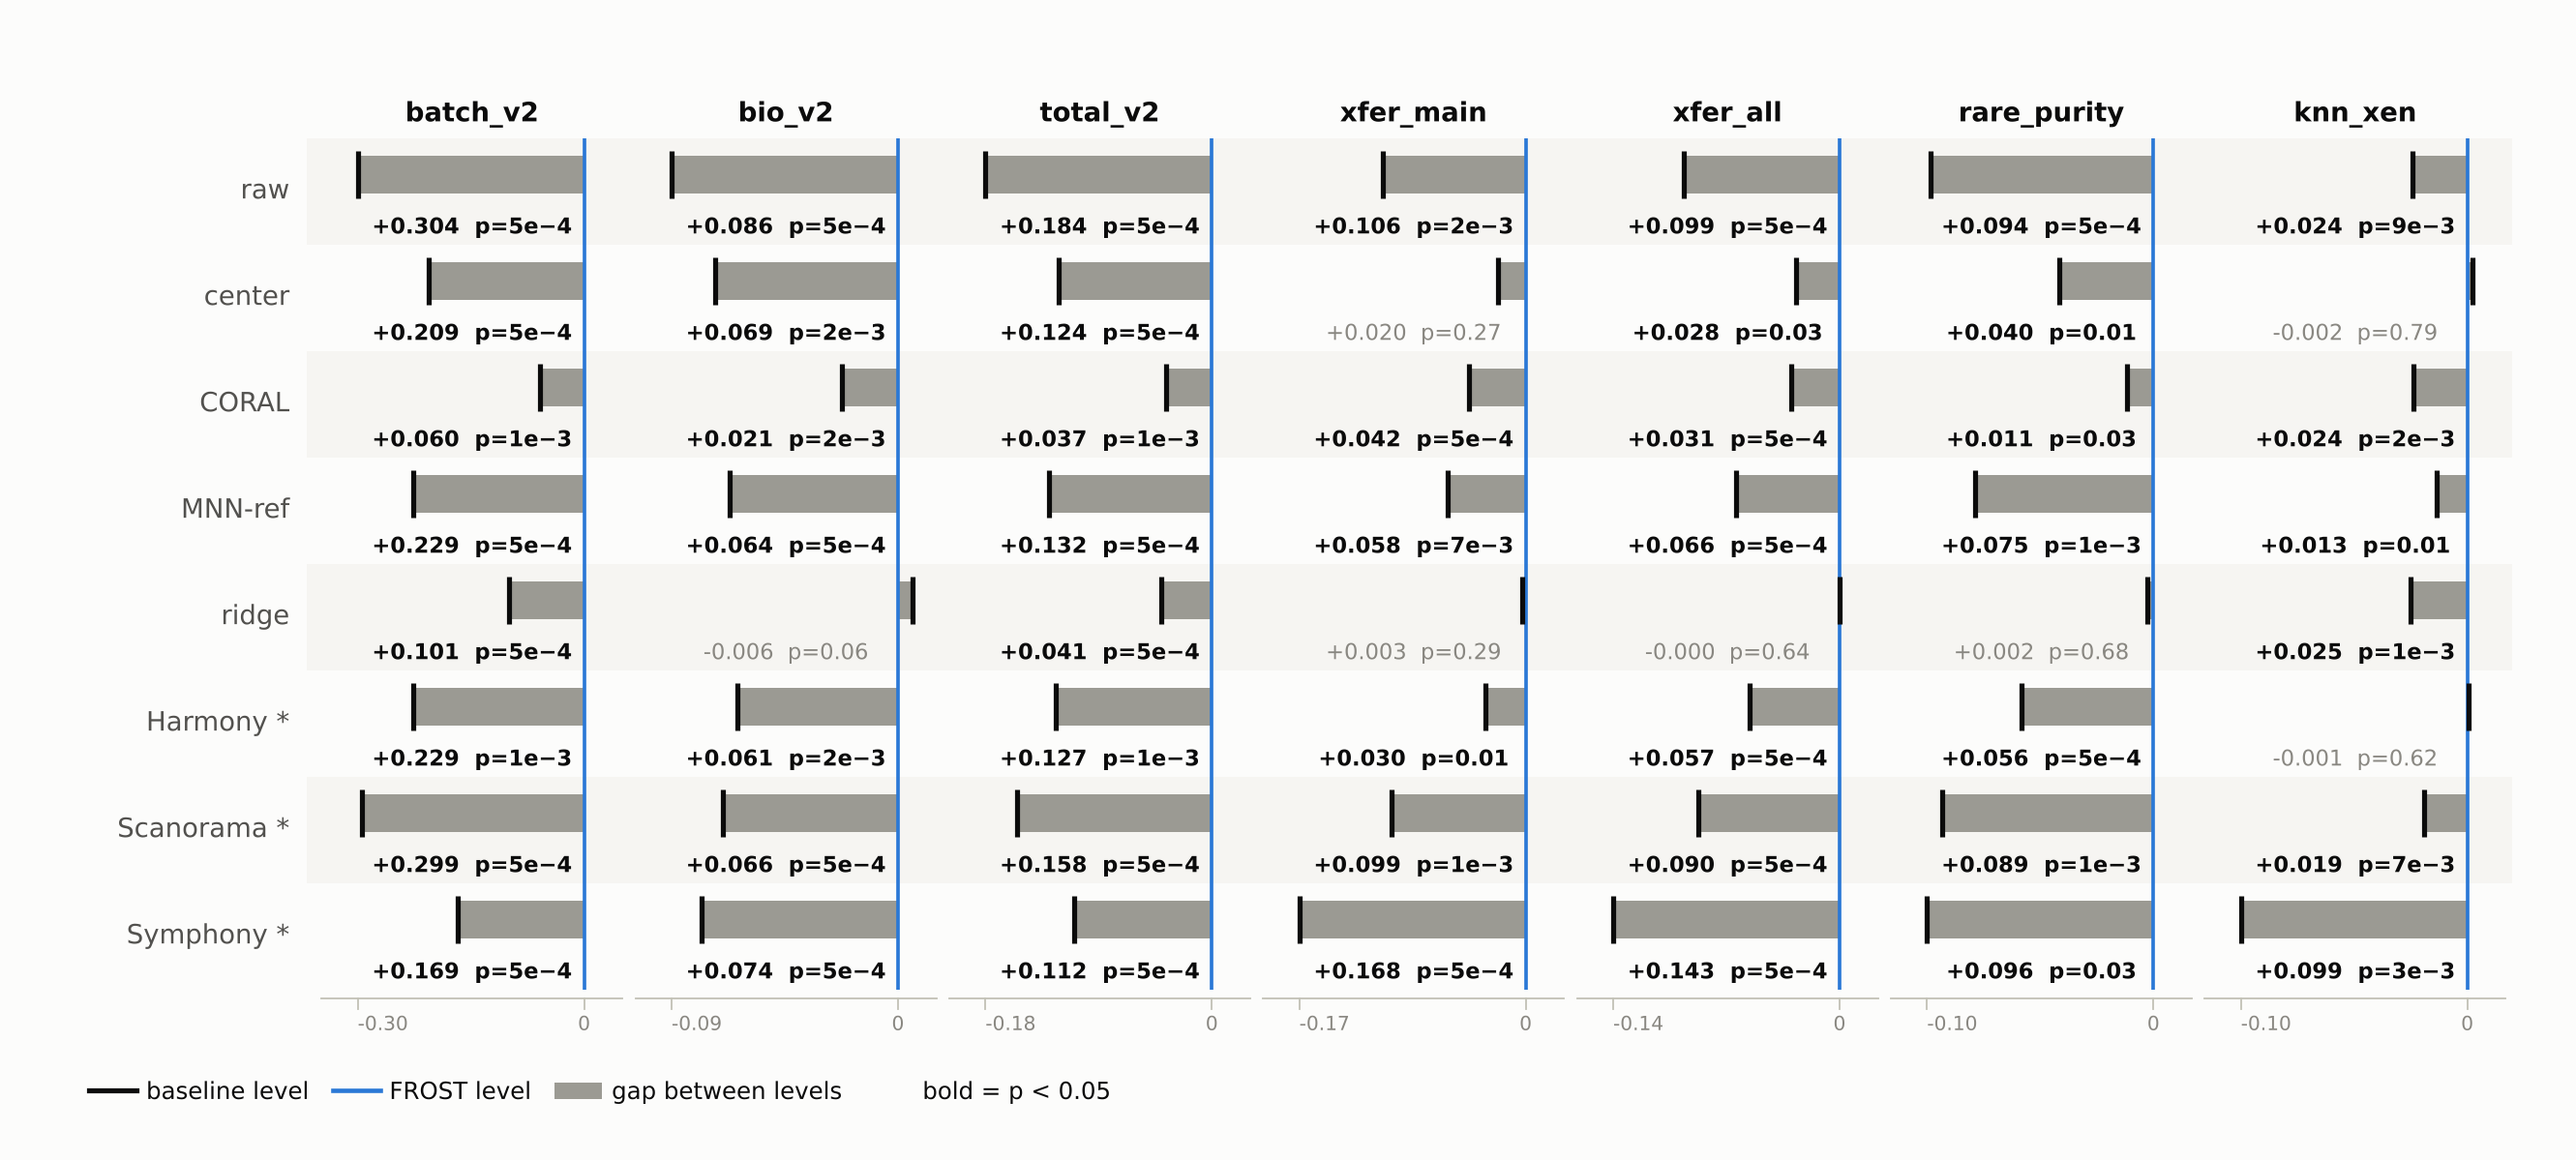
\includegraphics[width=\linewidth]{figs/fig_gaps.png}
\caption{Paired comparison of each baseline with \frost over 12 pairs. The blue line marks \frost; the black tick
marks the baseline, placed at minus the median of the 12 paired differences (\frost $-$ baseline). Bar, tick and
printed value all use that median, which is the quantity the Wilcoxon signed-rank test examines. Values in bold have
$p<0.05$. With 12 pairs $p$ cannot fall below $2/2^{12}\approx4.9\times10^{-4}$, and pairs within a tissue are
not independent, so $p$ describes consistency and the median describes magnitude. $^{*}$Methods that modify the
reference embedding.}
\label{fig:gaps}
\end{figure}

\subsection{Ablations}\label{sec:res_ablation}

\paragraph{Post-hoc moment matching.}\label{sec:res_coral}
On the common subsample, adding CORAL to USHER-ST (giving USHER-CC) raises mixing by $+0.191$ ($n=12$, $p=0.0015$)
and transfer by only $+0.0086$ (Table~\ref{tab:graphst}). On the main benchmark, \frost exceeds USHER-ST on
batch\_v2 ($p=0.0005$), total\_v2 ($p=0.0010$), xfer\_all ($p=0.0068$) and rare\_purity ($p=0.0024$), and does not
differ significantly on bio\_v2, xfer\_main or knn\_xen ($n=12$, except $n=11$ for xfer\_main). The two differ in
CORAL and in how the structure matrices are built; since the latter has no detectable effect (below), we attribute
the gain to CORAL. CORAL is thus justified on the cell-level metrics at no significant cost there. Its cost appears
at the gene level (Section~\ref{sec:limitations}).

\paragraph{Reference floor.}\label{sec:res_floor}
The per-class floor was fixed before evaluation, on a validation split of the training tiles. The rule was the
largest rare-type purity among floors that lost no more than 0.02 in xfer\_main or total score, with the 0.02
threshold set in advance. That rule chose 200. On held-out tiles, larger floors improve xfer\_main, xfer\_all and
rare-type purity slightly (Supplementary Table~\ref{tab:floor}), so 200 is conservative rather than tuned on
evaluation data.

\paragraph{Computational cost of the structure matrices.}\label{sec:res_cost}
Table~\ref{tab:cost} times three structure configurations on the four COAD pairs (seed 0, 25 EM iterations): the
adaptive landmark $\Cs$ of USHER-ST, a frozen exact $\Cs$ on the embeddings alone, and \frost's frozen exact $\Cs$
on augmented features. Freezing $\Cs$ cuts the number of $\Cs$ builds from 100 to 4, a 25-fold reduction equal
to the number of EM iterations. Each exact build is more expensive than a landmark one, but total $\Cs$ time still falls 2.7-fold,
and EM wall-clock time falls from 457.7\,s to 386.1\,s per pair. Adding the microenvironment block costs
nothing measurable (387.3\,s, with the same 8 builds). These diagnostic runs use 25 iterations, whereas the
benchmark maps use 10. The number of builds for the frozen configurations does not depend on the number of
iterations.

\begin{table}[t]
\centering
\caption{EM cost on the four COAD pairs (seed 0, 25 iterations). Wall-clock is real time. $\Cs$ time is thread
time summed over four worker threads; it is not real time and must not be added to wall-clock.}
\label{tab:cost}
\small
\begin{tabular}{@{}lccc@{}}
\toprule
 & landmark $\Cs$, recomputed & exact $\Cs$, frozen & \frost \\
\midrule
EM wall-clock, CosMx 6K (s)      & 431.7 & 355.4 & 361.7 \\
EM wall-clock, Visium HD FF (s)  & 462.0 & 404.5 & 385.8 \\
EM wall-clock, Visium HD FFPE (s)& 437.5 & 361.5 & 366.8 \\
EM wall-clock, Stereo-seq (s)    & 499.7 & 422.9 & 435.0 \\
EM wall-clock, mean (s)          & 457.7 & 386.1 & 387.3 \\
$\Cs$ builds                     & 100   & 4     & 4 \\
Total structure builds           & 104   & 8     & 8 \\
$\Cs$ thread time (s)            & 333.9 & 122.2 & 122.9 \\
\bottomrule
\end{tabular}
\end{table}

\paragraph{Structure matrices and the microenvironment term.}\label{sec:res_niche}
\frost and USHER-CC are indistinguishable on every metric: on the compact set, all $p\ge0.26$ ($n=12$), with no
median difference larger than 0.0008 in absolute value; on the common subsample, $p=0.75$ for transfer and $p=0.067$
for mixing. The difference measures the joint effect of three simultaneous changes to $\Cs$: adding the
microenvironment, replacing landmark distances with exact geodesics, and replacing per-iteration recomputation on
$f_\theta(\mathbf{X}^{s})$ with a single computation on the unmapped source. On the PCA pairs a fourth difference is
added: the 64-dimensional low-rank projection applies to the augmented features but not to the 50-dimensional
embeddings. We cannot separate the contribution of the microenvironment with the data at hand. What the frozen
construction does change is cost, as shown above.

\subsection{Comparison with USHER}\label{sec:res_usher}
Table~\ref{tab:usher} compares \frost with the unmodified USHER reference implementation on the four COAD pairs. With
four pairs and a single seed, no paired test can reach significance (exact two-sided floor $p=0.125$); we
therefore report differences descriptively. The two pipelines also differ in four components at once
(Table~\ref{tab:usher_vs_frost}), so this is a pipeline-level comparison, not an ablation.

The two methods sit at different points of the same trade-off, and their total scores are level (total\_v2 0.7055
for USHER, 0.7025 for \frost). USHER is higher on the mixing group score (batch\_v2 $-0.028$, \frost minus USHER);
\frost is higher on the conservation group score (bio\_v2 $+0.014$) and on every task metric, with the largest
differences on the three that probe rare types and local geometry: xfer\_all, rare-type purity and knn\_xen ($+0.034$ to $+0.038$). These are the metrics outside
USHER's own benchmark. Adding CORAL to USHER raises its mixing further without changing this pattern.

\frost reaches this point of the frontier at a fraction of the cost. USHER recomputes exact structure matrices
200 times per pair, against 8 for \frost ($2BT$ against $2B$ with $T=25$). USHER's EM took 2{,}570--3{,}219\,s per
pair (mean 2{,}911\,s), with 54--67\% spent building structure matrices. \frost took 361.7--435.0\,s (mean
387.3\,s) at the same number of iterations, about 7.5-fold less. Both ran on the same hardware type, but the timing
difference also includes the other three differences between the pipelines.

\begin{table}[t]
\centering
\caption{USHER reference implementation versus \frost, four COAD pairs. USHER: one seed, 25 iterations. \frost and
ridge: three seeds, means. The pipelines differ in four components (Table~\ref{tab:usher_vs_frost}). $\Delta$: \frost minus USHER. Imputation is
omitted because the archived values use the leaking protocol (Section~\ref{sec:limitations}).}
\label{tab:usher}
\small
\begin{tabular}{@{}llccccc@{}}
\toprule
Group & Metric & USHER & USHER + CORAL & \frost & ridge & $\Delta$ \\
\midrule
\multirow{6}{*}{Mixing}
 & iLISI        & 0.5551 & 0.6609 & 0.5261 & 0.2215 & -0.0290 \\
 & kBET         & 0.5153 & 0.5049 & 0.4440 & 0.1961 & -0.0713 \\
 & BRAS         & 0.8604 & 0.8387 & 0.8450 & 0.8502 & -0.0154 \\
 & graph conn.  & 0.9768 & 0.9747 & 0.9800 & 0.9796 & +0.0032 \\
 & batch ASW    & 0.9268 & 0.9147 & 0.9152 & 0.9196 & -0.0116 \\
 & batch\_v2    & 0.7269 & 0.7448 & 0.6987 & 0.5618 & -0.0282 \\
\midrule
\multirow{6}{*}{Conservation}
 & NMI          & 0.6411 & 0.6412 & 0.6780 & 0.6739 & +0.0369 \\
 & ARI          & 0.6442 & 0.6461 & 0.6828 & 0.6924 & +0.0386 \\
 & ASW          & 0.5924 & 0.5852 & 0.5826 & 0.5904 & -0.0098 \\
 & cLISI        & 0.9837 & 0.9891 & 0.9935 & 0.9939 & +0.0098 \\
 & iso.\ labels & 0.5950 & 0.5896 & 0.5884 & 0.5951 & -0.0066 \\
 & bio\_v2      & 0.6913 & 0.6902 & 0.7050 & 0.7091 & +0.0137 \\
\midrule
Total & total\_v2 & 0.7055 & 0.7120 & 0.7025 & 0.6502 & -0.0030 \\
\midrule
\multirow{4}{*}{Tasks}
 & xfer\_main   & 0.7052 & 0.6965 & 0.7090 & 0.7091 & +0.0038 \\
 & xfer\_all    & 0.4336 & 0.4405 & 0.4715 & 0.4663 & +0.0379 \\
 & rare\_purity & 0.2610 & 0.2803 & 0.2990 & 0.2909 & +0.0380 \\
 & knn\_xen     & 0.4119 & 0.4036 & 0.4456 & 0.4200 & +0.0337 \\
\bottomrule
\end{tabular}
\end{table}
